\documentclass{ctexart}
\usepackage{amsmath}
\usepackage{amsfonts}
\def\dd{{\rm d}}
\def\ee{{\rm e}}
\def\vec#1{\mathbf{#1}}
\begin{document}
\title{计算物理作业 16}
\author{刘畅\qquad PB09203226}
\maketitle

{\bf [作业16]}: 设体系的能量为 $H = \frac{x^2}{2\sigma_x^2} +
\frac{y^2}{2\sigma_y^2}$ (以 $kT$ 为单位), 采用 Metropolis 抽样法
计算 $\langle x^2\rangle$, $\langle y^2\rangle$, $\langle x^2+y^2\rangle$,
并与解析结果进行比较. 抽样时在 2 维平面上依次标出Markov 链点分布, 从而形象地理解Markov链.

\section{算法}
由于做一个(线性的)变量代换
\begin{align*}
x&\to x/\sigma_x\\
y&\to y/\sigma_y
\end{align*}
就可以变到题目中的情形, 因此设 $\sigma_x = \sigma_y = 1$ 并不会影响一般性. 所以我们
下面都采取这样的假定. 由于 $H$ 用 $kT$ 做单位, 因此 $\beta = 1$, 正则系综的配分函数
为
\[
Z = \int_{\mathbb{R}^2} \ee^{-H} \,\dd x\,\dd y=\int^{+\infty}_{-\infty}\dd x\int^{+\infty}_{-\infty}\dd y\,\ee^{-\frac{x^2}{2}-\frac{y^2}{2}}= 2\pi
\]
这样系统处于态 $(x,y)$ 的概率密度是
\[
p(x,y) = \frac{\exp\left(-\frac{x^2}{2}-\frac{y^2}{2}\right)}{2\pi}
\]
因此 $x^2$, $y^2$, $x^2+y^2$ 理论上的平均值为
\[
\langle x^2\rangle = \int_{\mathbb{R}^2}p(x,y)x^2\,\dd x\,\dd y = 1
\]
同理
\begin{align*}
\langle y^2\rangle = 1\\
\langle x^2+y^2\rangle = 2
\end{align*}
容易看出在 $\sigma_x\neq1$, $\sigma_y\neq1$ 的单位下上面的结果是
\begin{align*}
\langle x^2\rangle &= \sigma_x^2\\
\langle y^2\rangle &= \sigma_y^2\\
\langle x^2+y^2\rangle &= \sigma_x^2 + \sigma_y^2
\end{align*}

按照书上的算法, Metropolis 算法的步骤是
\begin{enumerate}
\item 选择一个初始构形 $\vec R_0 = (x_0,y_0)$
\item 在 $[-h,h]\times[-h,h]$ 区间内的均匀分布中随机选择一个点作为 $\Delta\vec R$,
计算新的构形 $\vec R'$.
\item 计算新的构形和旧的构形在正则分布概率密度下出现的概率的比值
\[
\eta = \frac{p(x',y')}{p(x,y)}
\]
\item 随机抽取 $[0,1]$ 上的均匀分布 $w$, 如果 $\eta > w$, 那么 $\vec R_{i+1} =
\vec R'$, 否则 $\vec R_{i+1} = \vec R_i$.
\item 重复直到足够多步
\end{enumerate}

最后得到的点列 $\vec R_i$ 中, 为了减少误差, 通常舍去前面的一些点, 同时为了减少
自相关系数的影响, 中间要跳过一些点, 最后得到 $f(\vec r)$ 的值为
\[
\langle f\rangle = \sum_{i=0}^{\rm nsteps} f(\vec R_{n_0+i\cdot n_d})
\]
\section{程序}
按照惯例, 用一个结构来表示点 $(x,y)$:
\begin{verbatim}
struct point {
    double x, y;
};
\end{verbatim}

\verb|rand_norm()| 和 \verb|rand_unif()| 是两个均匀分布的抽样函数, 前面
的作业用过好多次了. 由于前面的算法中只要用到 $p(x,y)$ 的相对值, 因此 $\frac{1}{2\pi}$
系数是不需要的. $p(x,y)$ 函数实现在 \verb|prob_dist()|:
\begin{verbatim}
/* Probability distribution for our canonical ensemble with
 * Hamiltonian H(x,y) = x^2/2 + y^2/2
 */
double prob_dist(struct point p)
{
    return exp(-p.x*p.x/2 - p.y*p.y/2);
}
\end{verbatim}

\verb|generate_new_configuration()| 函数用来实现算法的主要部分: 从旧的构形生成
新的构形, 就是把前面的算法翻译成C 语言, 这个没有什么好解释的:
\begin{verbatim}
/* generate a new configuration based
   upon the above accepting criterion */
struct point generate_new_configuration
                 (double h, struct point old)
{
    double p;
    struct point new;
    double x = rand_unif(h);
    double y = rand_unif(h);
    new.x = old.x + x;
    new.y = old.y + y;
    p = prob_dist(new) / prob_dist(old);
    if (is_accepted(p))
        return new;
    else
        return old;
}
\end{verbatim}
其中 \verb|is_accepted()| 例程实现上面算法中的舍选.

最后只需要有选择地把 $\vec R_i$ 处的值加起来就得到了 $\langle f\rangle$.
这段代码在 \verb|metropolis()|. 这代码中唯一需要解释的是宏 \verb|spit_all()|
和 \verb|spit_hit()|. 前者用来把每个 $\vec R_i$ 输出到文件, 后面把求
$\langle f\rangle$ 用到的 $\vec R_i$ 输出到文件.

\section{结果}
程序运行的结果为:
\[
\input res_x2
\]
\[
\input res_y2
\]
\[
\input res_x2_y2
\]
可以看到和理论值是非常接近的.
每一步 Markov 链的图为:
\begin{center}
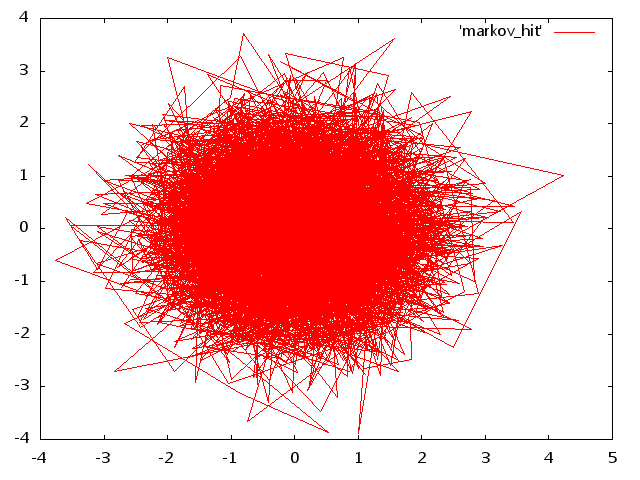
\includegraphics[width=4in]{markov_hit.png}
\end{center}
这是 \verb|spit_hit()| 的输出.
\begin{center}
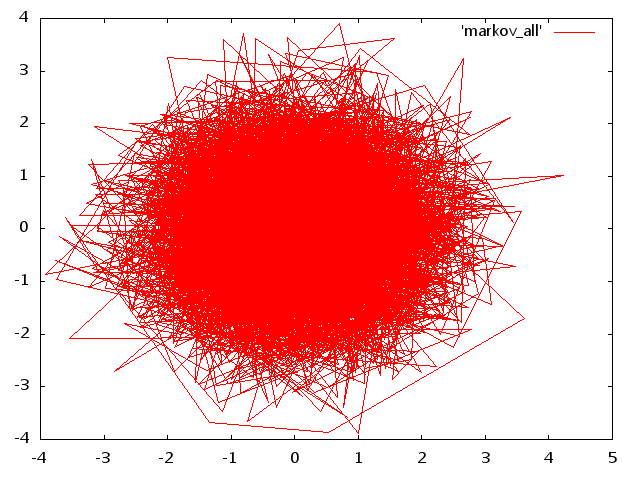
\includegraphics[width=4in]{markov_all.png}
\end{center}
这是 \verb|spit_all()| 的输出.

\end{document}